\documentclass[Bachelorarbeit.tex]{subfiles}

%Implementation issues (document only what is not documented in the selected literature, but necessary for implementation, e.g. software structure…)

\begin{document}
\chapter{Implementation issue}
\section{Color based face detection on a picture}
To load an image into the workspace and find suitable thresholds in the YCbCr space the informations from the lecture Color in the course Image and Signal Processing (\cite{RobAmaColor}). A detailed description to this procedure can be found in the attachment \ref{sec:ColorThre}

\medskip
The thresholding itselve can be done by logical operations like in the listening \ref{matlabColorTresholdingDetail}.

\begin{lstlisting}[caption=Color thresholding, label= matlabColorTresholdingDetail]
% Thresholding -> binary
thresh_cb = cb > 105 & cb < 120;    % thresholding for cb values
thresh_cr = cr > 140 & cr < 165;    % thresholding for cr values
binary_pic = thresh_cb&thresh_cr;   % create binary picture
\end{lstlisting}

\medskip
To detect faces out of the binary image (to reject areas/bolobs which are no faces) a few process steps are necessary. The process is described in the article \cite{RTFaceDetection}, for this steps MATLAB-Functions are available which looks like listening \ref{RejectionOfNonSkinRegion}.
\begin{lstlisting}[caption=Rejection of non Face Skin Region , label= RejectionOfNonSkinRegion]
%label all the connected components in the image
bw=bwlabel(close_binary_pic,8);

%image blob analysis - we get a set of properties for each labeled region
area=regionprops(bw,'Area')                    
eulernumber=regionprops(bw,'EulerNumber');      
eccentricity=regionprops(bw,'Eccentricity');    
centroid=regionprops(bw,'Centroid');            
boundingbox=regionprops(bw,'BoundingBox');
\end{lstlisting}

The whole script can be found in the attachment xx.



\section{Color based face detection on a video}



\section{Color based face detection on a Raspberry Pi}

\subsection{Simulink Model - Face detection on an image}
The \textit{Image Processing Toolbox } from Simulink provides the function to load an image from a file, convert this imager (from RGB) into the YCbCr space, make the blob analysis, draw the rectangular (which represents a detected face) on the image and display the image on a figure. 

To threshold the YCbCr image a MATLAB-function block (\textit{color thresholding} in figure \ref{SimulinkImage}) was inserted. The MATLAB-function block \textit{remove misshapen skin regions} is used to remove rectangles which are wider than height (with this functions skin regions from hands can be rejected). This function block was necessary because the Blob Analysis block didn't support all necessary functions (for example the eulernumber is missing).
\begin{figure}[!h]
\centering
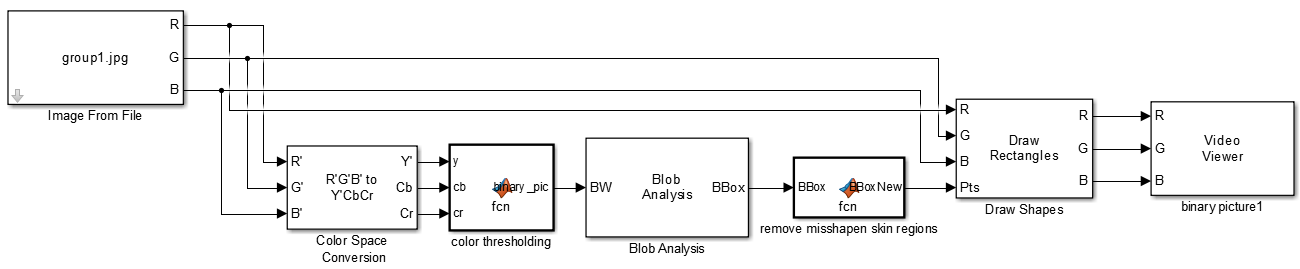
\includegraphics[width=14cm]{./img/simulink/Simulink_ImageProcessing.PNG} 
\caption{Simulink model - Face detection on an image}
\label{SimulinkImage}
\end{figure}

The code of the Matlab function blocks can be found in the attachment \ref{sec:SimulinkFaceImage}.


\subsection{Simulink Model deployed on Raspberry Pi with I/O connection to the host PC}

To run a Simulink model on a Raspberry Pi the hardware support package Run models on Raspberry Pi is necessary. The package installation hints and Examples can be found on \href{https://de.mathworks.com/hardware-support/raspberry-pi-simulink.html}{Raspberry Pi Support from Simulink}. 

\medskip
Hints to run a Simulink block on the Raspberry Pi:
\begin{itemize}
\item Use a standalone licence or a network licence without VPN. By using a licence over a VPN it is not possible to communicate with the Raspberry Pi.
\item Before using the Raspberry Pi camera module the steps from the instructions \href{https://de.mathworks.com/help/supportpkg/raspberrypi/ug/add-support-for-raspberry-pi-camera-board.html}{Use Camera Board with V4L2 Video Capture Block} must be done. Otherwise the Simulink block will not find the camera module.
\end{itemize}


\medskip
In a first step the setup looks like figure \ref{SimModelWithIO}. The idea is to get familiar with the Raspberry Pi camera module (the resulution, brightness, ...) and use the data for adjustments (especially for find suitable thresholds). In this case the model should run in the external mode, the instructions \href{https://de.mathworks.com/help/supportpkg/rtlsdrradio/ug/run-model-in-external-mode.html}{Run Model in External Mode} provides all necessary informations.

\begin{figure}[!h]
\centering

\includegraphics[width=5cm]{./img/Under_construction.JPG} 
\caption{Simulink model setup - With I/O connection to the host}
\label{SimModelWithIO}
\end{figure}

The Simulink model itself was built up similar with the model in figure \ref{SimulinkImage}, see figure \ref{SimModelRaspIO}.
\begin{figure}[!h]
\centering
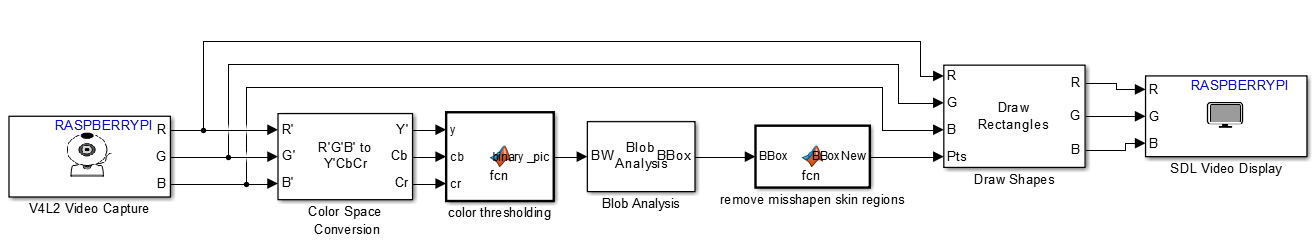
\includegraphics[width=14cm]{./img/simulink/Simulink_RaspberryPi.PNG} 
\label{SimModelRaspIO}
\caption{Simulink model - With I/O connection to the host}
\label{SimModelWithIO}
\end{figure}

\subsection{Simulink Model as Standalone Application}
The final step is to deploy the on the hardware. As model the model of figure \ref{SimModelRaspIO} is used. To deploy the model on the hardware the instruction \href{https://de.mathworks.com/help/supportpkg/rtlsdrradio/ug/run-model-as-standalone-application.html}{Run Model as Standalone Application} is useful.

\begin{figure}[!h]
\centering

\includegraphics[width=5cm]{./img/Under_construction.JPG} 
\caption{Simulink model setup - Standalone application}
\label{SimModelWithIO}
\end{figure}




\end{document}
